% Slide 4 -- the conceptual pivot, as three relations rather than three bullets.
%
% The paper's foundation sentence: a chronological split is a predicate over the rows of ONE
% realised dataset, and the four gaps are not. Each has a counterexample that exists only in
% another execution, another source state, or another aggregation level. Those are the three
% panels below, in that order, and the caption names what they have in common.
%
% WIDTH. Must stay inside ~140mm: the first version ran to 191mm and the third panel was simply
% off the slide. Rendering caught it; the source looked fine.
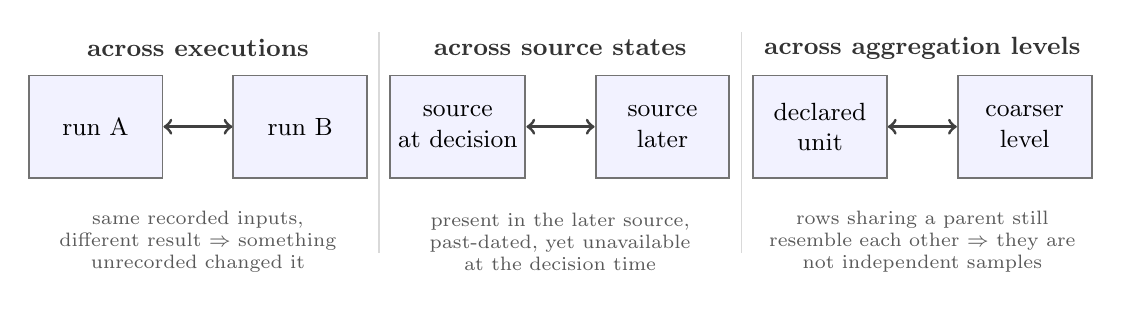
\begin{tikzpicture}[
  x=1mm, y=1mm, font=\footnotesize,
  box/.style={draw=black!55,line width=0.7pt,fill=blue!5,minimum width=17mm,
              minimum height=13mm,align=center,inner sep=1mm,font=\small},
  rel/.style={<->,line width=1.1pt,black!75},
  note/.style={font=\scriptsize,text=black!65,align=center,text width=40mm,minimum height=11mm,anchor=north},
  hdr/.style={font=\small\bfseries,text=black!80,align=center}]

\node[hdr] at ( 21.5,30) {across executions};
\node[box] (a1) at (  8.5,20) {run A};
\node[box] (a2) at ( 34.5,20) {run B};
\draw[rel] (a1) -- (a2);
\node[note] at ( 21.5,11) {same recorded inputs,\\different result $\Rightarrow$ something\\unrecorded changed it};

\draw[black!15,line width=0.5pt] (44.5,32) -- (44.5,4);

\node[hdr] at ( 67.5,30) {across source states};
\node[box] (b1) at ( 54.5,20) {source\\at decision};
\node[box] (b2) at ( 80.5,20) {source\\later};
\draw[rel] (b1) -- (b2);
\node[note] at ( 67.5,11) {present in the later source,\\past-dated, yet unavailable\\at the decision time};

\draw[black!15,line width=0.5pt] (90.5,32) -- (90.5,4);

\node[hdr] at (113.5,30) {across aggregation levels};
\node[box] (c1) at (100.5,20) {declared\\unit};
\node[box] (c2) at (126.5,20) {coarser\\level};
\draw[rel] (c1) -- (c2);
\node[note] at (113.5,11) {rows sharing a parent still\\resemble each other $\Rightarrow$ they are\\not independent samples};
\end{tikzpicture}
